\section{Matrices usage example}

In this section we present an insurance company's service that manage insurance contracts to demonstrate how the presented comparison matrices can be used in a real-world context. The domain of the project we present here is a lighten version of the combination of domains from projects we have done at FABERNOVEL for former clients, who are big french insurance companies.

\subsection{Domain description}

To manage insurance contracts, the service holds five kinds of resources: (i) third-parties, (ii) contracts, (iii) warranties, (iv) cases and (v) services. Third-parties, who can for example be customers or contractors, enter into contracts with the insurance company. These contracts include warranties from the closed list of warranties that the company offers. Each warranty has options, let's take for example Person A who has the following warranties: (i) damage coverage with a deductible of \$500, and a maximum repair amount of \$30.000, (ii) premium vehicle loan in the event of immobilization of the damaged vehicle and (iii) reimbursement of the transport to the destination in the event of an accident, capped at \$2.000. A contract can have several cases. When an insured has a claim the company creates a case that holds the claim details and the services provided to the insured. For example, Person A has a car accident, he opens the insurance's web application and report a claim, which leads to the company opening a case. His car has been destroyed and he is expected to attend a family diner. So, on the app, he asks for a transport to his destination and a vehicle loan he will take delivery of at his destination the day after.

\subsection{Constraints on the technologies to select}

The service we describe have to communicate with both internal and external components. Internal components are front-end applications, such as mobile or web applications, and other kernel services, such as payments. External components are contractors APIs, for example taxi or mechanics companies. 

In the context of this service, there is a huge amount of business rules that determine (i) the warranties an insured can include in a contract and (ii) the available services for a case, based on the specificity of the given case and the warranties of the contract that the case is linked to. Writing and maintaining these rules both on the server and its clients would have been very costly. To keep business rules on the server-side only we decided to use the Hypermedia As The Engine Of Application State.

Because the project constitutes the core of the company's business, it should be future proof. We believe that this includes being Linked Data compatible because of the growing interest in those technologies and the new possibilities it offers, such as automatic mash-ups. Moreover, considering that the contractors that provide services are very diverse and numerous, the interactions with their APIs should leverage the possibilities offered by the use of RDF semantics, such as automatic discovery and composition. So, we looked for RDF-compatible technologies.
% [] - Explain why being future proof means being Linked Data compatible with one argument.

Because the project is core to the company, API clients will likely be built later on. So, the API should document its resources, resources' attributes, operations, URI templates, HTTP verbs, hypermedia controls and errors in a machine-interpretable way. Moreover, because the service applies the CQRS pattern\footnote{\url{https://martinfowler.com/bliki/CQRS.html}} we needed the IDL to allow associating each operation to its own input and output data model.

In the category of interchange format, the goal was to be as close as possible to what developers already know. So the format had to be based on JSON and entity-centric. The structure had to be as close as possible to an original JSON document.

Last, frameworks were considered based on the level of automation they provide.

\subsection{Selection of the technologies}

From these constraints we select a set of criteria and features to look for, which are checked on Fig~\ref{idl-matrix}, Fig~\ref{interchange-formats-matrix}, Fig~\ref{frameworks-matrix}. We then count how many of these criteria each technology meet. Results are presented in Fig~\ref{example-idl-results}, Fig~\ref{example-dif-results} and Fig~\ref{example-frameworks-results}. For each kind of technology, the three technologies matching the highest amount of selected criteria are highlighted in green.

\begin{figure}[ht]
\caption{Results for interface description languages}
\centering
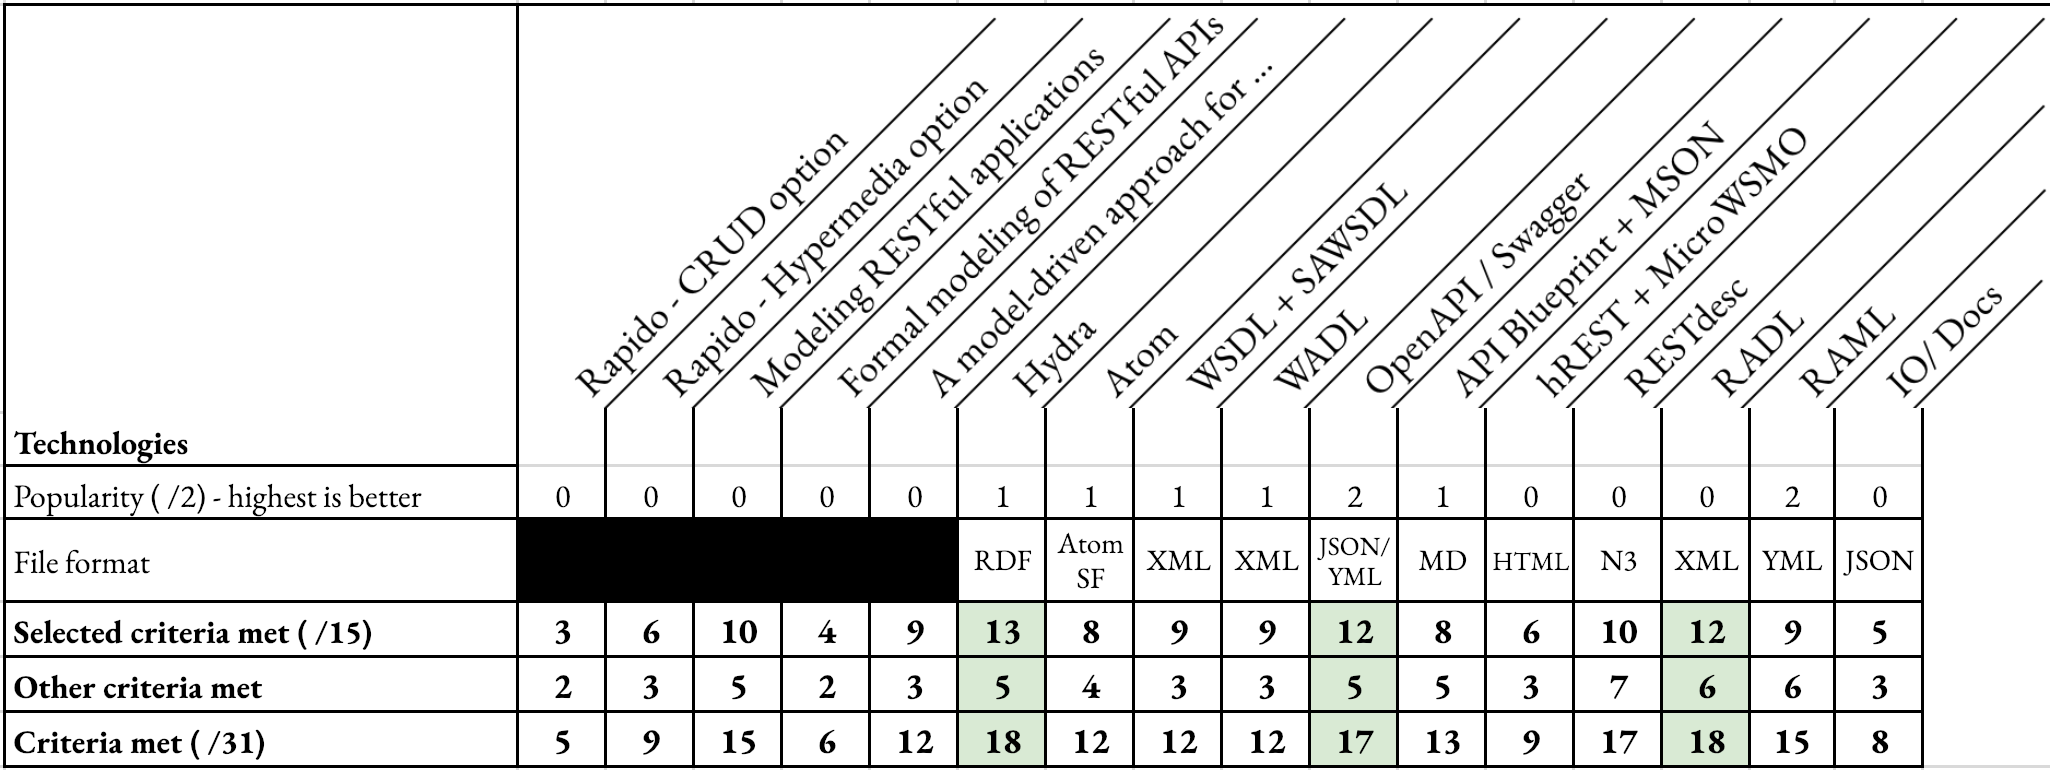
\includegraphics[width=0.8\textwidth]{figures/example-idl-results.png}
\label{example-idl-results}
\end{figure}

\begin{figure}[ht]
\caption{Results for data interchange formats}
\centering
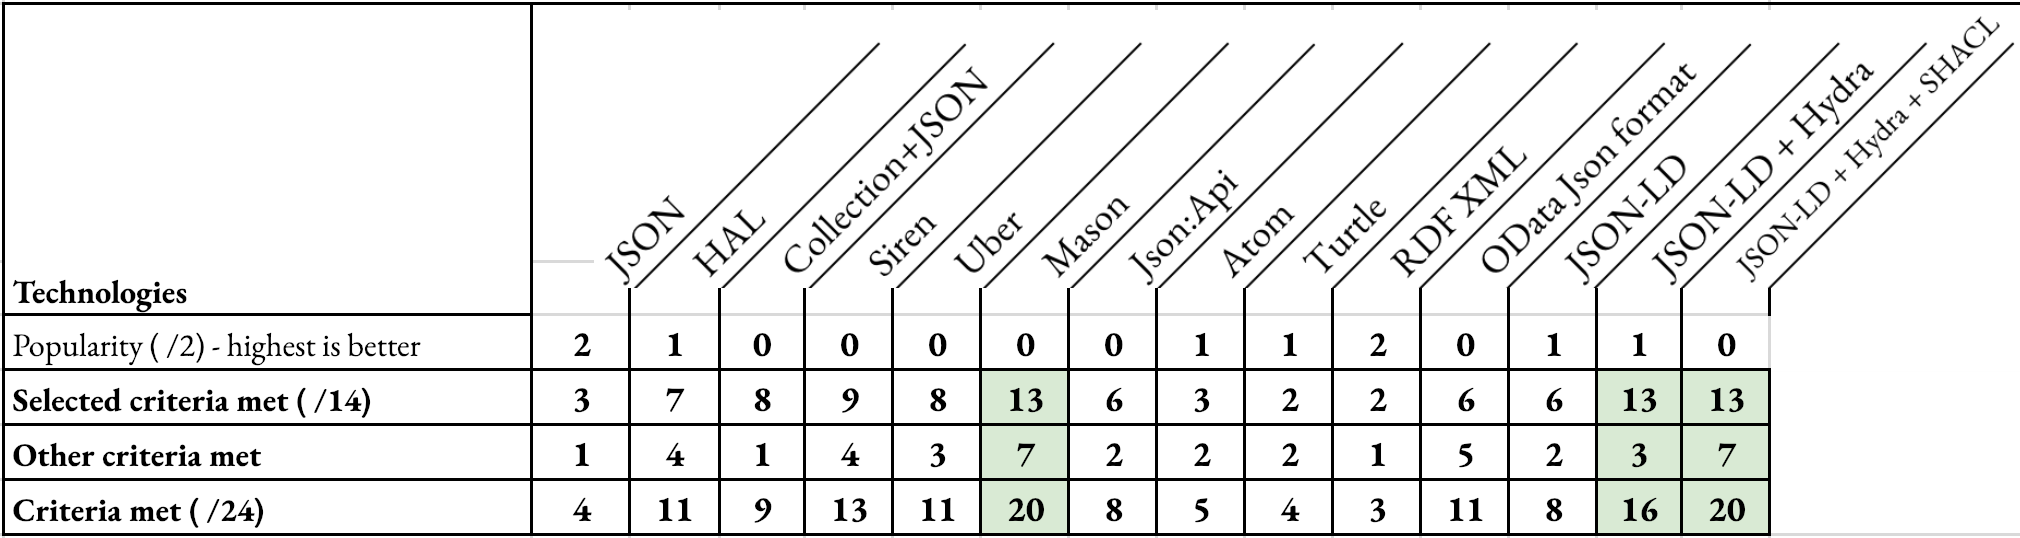
\includegraphics[width=0.8\textwidth]{figures/example-dif-results.png}
\label{example-dif-results}
\end{figure}

\begin{figure}[ht]
\caption{Results for implementation frameworks}
\centering
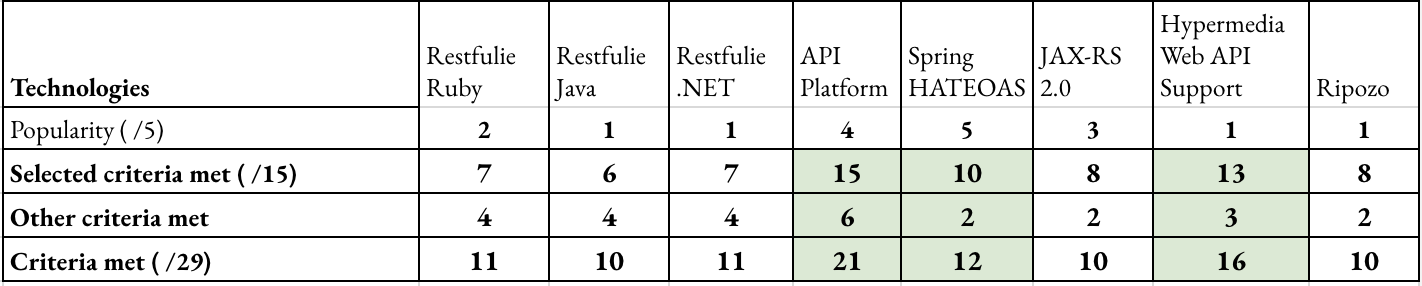
\includegraphics[width=0.8\textwidth]{figures/example-frameworks-results.png}
\label{example-frameworks-results}
\end{figure}

Technologies don't have to match every criteria to be selected. Most of the time, missing features can be implemented afterwards, or proposed to the maintainers of the technologies. A fine-grained analysis should be done on a per-feature basis.

\textbf{Interface Description Language.} Hydra, OpenAPI and RADL are the three technologies matching the highest number of selected criteria. However, no one matches every criteria. Hydra lacks the ability to describe non-functional properties and media-types, which can be done with other RDF vocabularies. RADL lacks the ability to semantically describe resources model and operations, errors and non-functional properties, which can also be done with other RDF vocabularies. On the other hand, OpenAPI does not support the description of hypermedia controls neither the usage of any RDF vocabulary, which is far more difficult to compensate. 

In the context of this project we chosen to use both Hydra and OpenAPI. OpenAPI because it has most features and is a must-have today because of its tooling and popularity. Hydra because it can be easily completed with other vocabularies and used with JSON-LD, when RADL is tight to XML.

\textbf{Interchange Formats.} Mason, JSON-LD + Hydra are the two technologies matching the highest number of selected criteria. JSON-LD + Hydra + SHACL can be ignored as it does not match more selected criteria than without SHACL. While JSON-LD + Hydra lacks the ability to describe non-functional properties, Mason does not allow to use RDF vocabularies. Again, being not compatible with RDF requires a lot more effort to compensate than finding another vocabulary. This explains why JSON-LD + Hydra was preferred over Mason in this context.

\textbf{Implementation frameworks.} API Platform, Spring HATEOAS and Hypermedia Web API Support \cite{salvadori2014framework} are the three technologies matching the highest number of criteria. Hypermedia Web API Support is immediately removed from the candidates because no public implementation is available. API Platform should be preferred over Spring HATEOAS because it matches five more criteria than Spring. However, developers of the companies we worked with know Java and not PHP. Moreover the Spring framework has a very good popularity with them which compensates the need to develop some features by hand. This is why we decided to go with Spring HATEOAS.

\subsubsection{Easing the selection of the technologies}

To ease the selection of the technologies with the comparison matrices, we developed an open-sourced web application\footnote{\url{https://antoinecheron.github.io/morice/}}. Users go through three steps: (i) selecting the kind of technologies they are looking for, (ii) selecting the criteria that are required and giving each criteria a value and then (iii) he is presented the results. Results is one table per kind of technology. In the table, the listed technologies are the ones that match the criteria that the user selected as required. Technologies are ranked by score. The score of one technology is the sum of the value of the criteria the technology meets.

% This tool is intended to be improved in future works.